\section{Methodology}
In this chapter, we let the user steer with motor imaginary brain signals the Cartesian position $x \in \mathbb{R}^2$ of the end-effector (i.e., the platform) of a planar \gls{HSA} robot.
We realize this strategy by first classifying the motor imaginary signals into Cartesian-space movement directions (e.g., the active axis and sign of the movement). We use this information to adjust the position of a task-space attractor iteratively (see Section~\ref{sub:braincontrol:planning_attractors_switching}). % Section~\ref{sub:braincontrol:computational_controller} describes how a model-based computational controller establishes this attractor. Importantly, we preserve the soft robot's compliance by shaping the closed-loop system's impedance in Cartesian space.
We illustrate the methodology in Fig.~\ref{fig:braincontrol:control_scheme}.

\begin{figure}
    \centering
    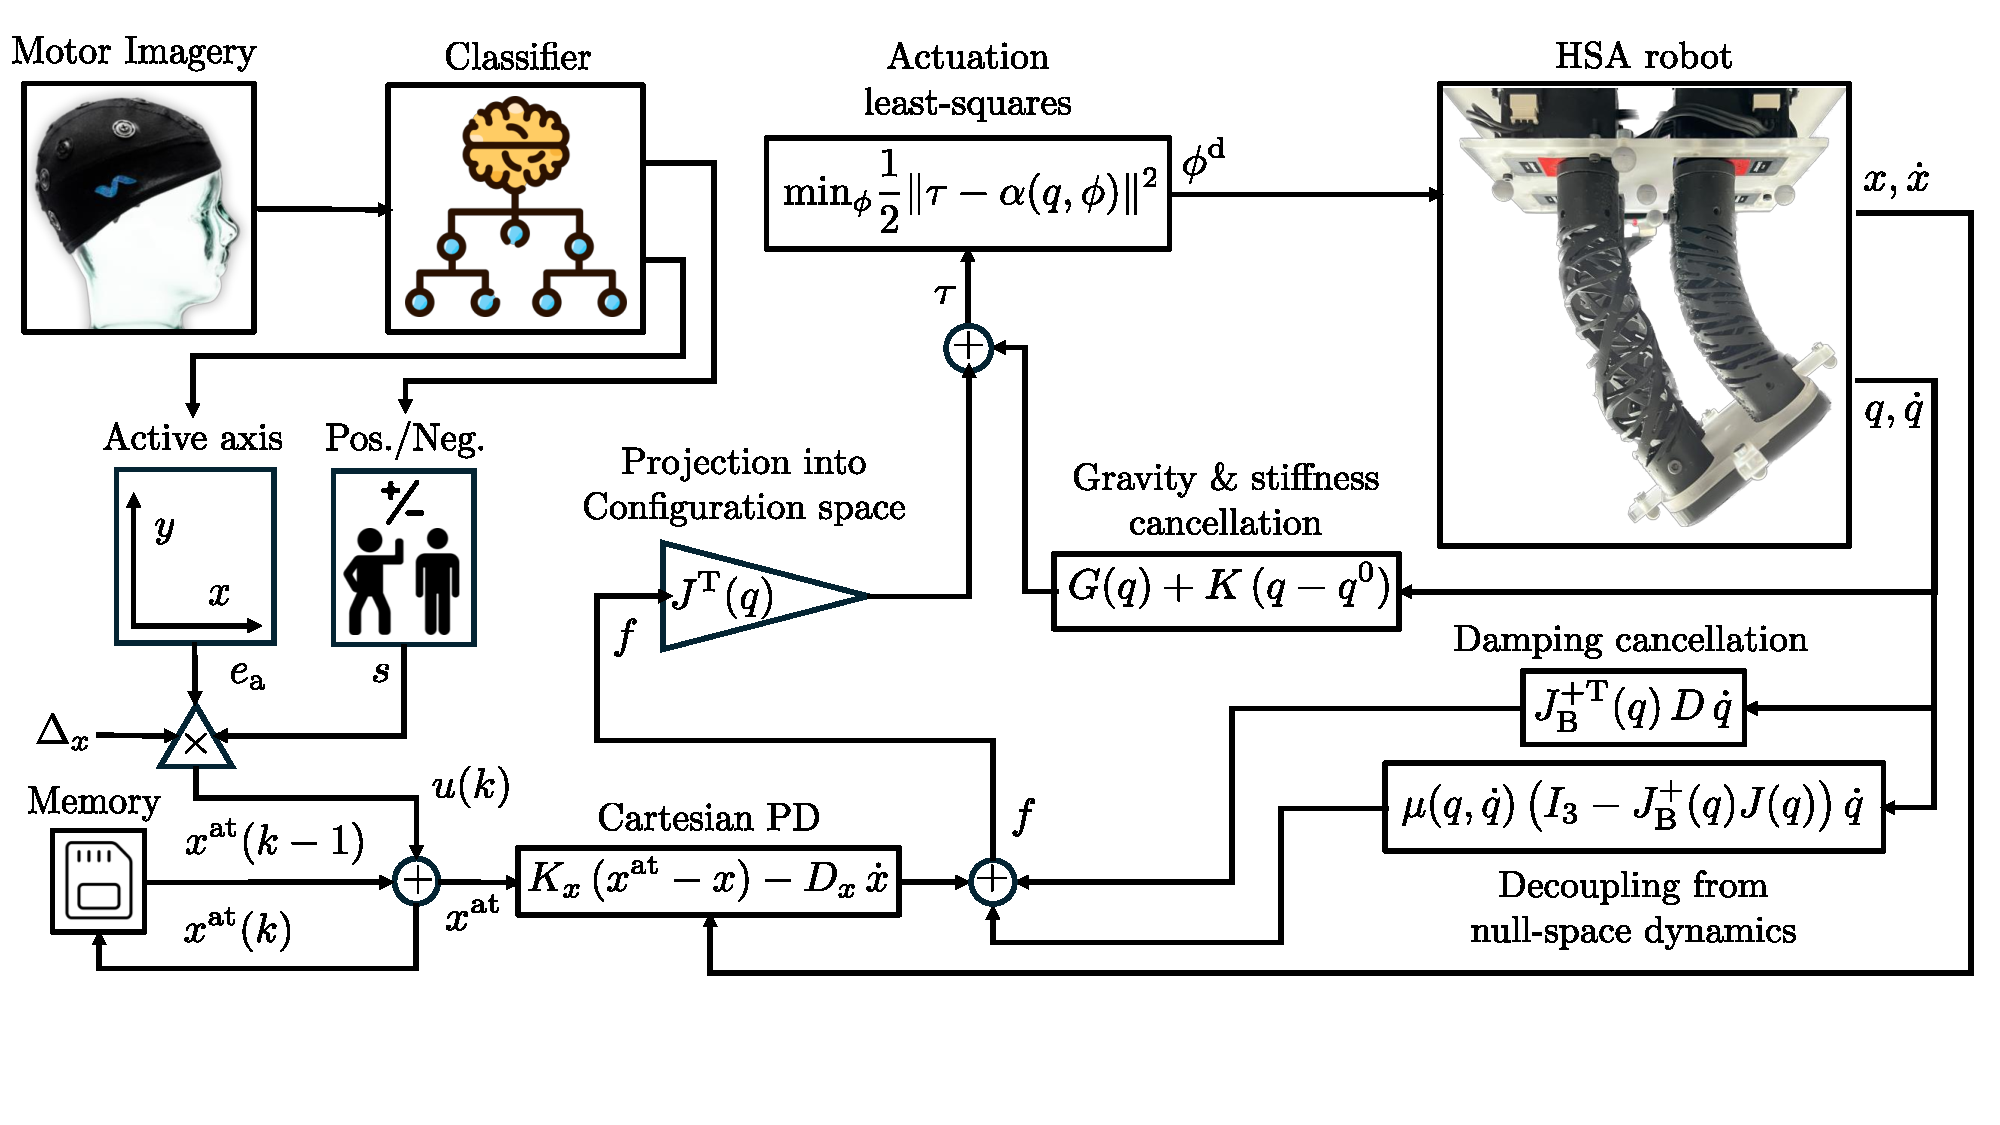
\includegraphics[width=0.95\textwidth]{braincontrol/figures/control_scheme/control_scheme_v2_cropped.pdf}
    \caption{Scheme of the proposed approach to control HSA robots with motor imagery. Brain signals steer an attractor in operational space: first, we switch the active coordinate axis when we detect jaw clenching. If no jaw clenching is detected, we classify the EEG signals based on left/right motor imaginations into positive and negative movements along the active axis. Next, we regulate the robot towards the chosen attractor position $x^\mathrm{at}$ with a Cartesian impedance controller. This controller first cancels all static forces and the residual coupling of the null space on the operational space dynamics. This allows us to now shape our own potential with a PD term in operational space. As the robot is underactuated, we optimize least-squares to identify the actuation $\phi^\mathrm{d}$ so that the residual between the desired and actual torques in the configuration space is minimized. Icons created by Flaticon\copyright.}
    \label{fig:braincontrol:control_scheme}
\end{figure}

\subsection{Background: Motor Imagery-based BMI systems}\label{sub:braincontrol:motor_imagery_bmi}

Imagining the movement of body parts or limbs (e.g., hands, legs, tongue) without moving it or the mental rehearsal of a motor act without overt movement execution is termed Motor Imagery~\citep{lotze2006motor}.  The neuronal activities observable inside a frequency range of \SI{8}{Hz} to \SI{12}{Hz} (Mu) and \SI{12}{Hz} to \SI{30}{Hz} (Beta) are associated with cortical areas directly connected to the brain’s motor output (activating primary sensorimotor areas that can be modulated with imaginary mental movement in healthy as well people with neuromuscular disabilities). 
% Motor Imagery is widely used for the BMI systems involved in either task-specific for instance exoskeleton /cite!!, or motion wheelchair /cite!!.

The motor imagery \gls{BMI} framework typically consists of four integral components:

\begin{enumerate}
    \item \textbf{Signal acquisition:} The initial stage involves the recording of neural signals while the person imagines the movements of the limbs, generally acquired using noninvasive methodologies (e.g., \gls{EEG}).
    \item \textbf{Feature extraction:} Following signal acquisition, signal processing techniques are applied to extract salient features from the neural patterns associated with specific cognitive processes or intentions.
    \item \textbf{Feature translation:} This translation phase interprets the user's cognitive intent, converting it into actionable instructions for external devices.
    \item \textbf{Device output:} The culmination of the \gls{BMI} process is the application of the interpreted commands to external devices. 
    % \glspl{BMI} can be employed in various applications, ranging from motor control tasks, such as wheelchair navigation, to text input and the orchestration of complex robotic exoskeletons.
\end{enumerate}

As detailed further in Sec.~\ref{sub:braincontrol:bmi_protocol}, we leverage the difference in signals when imagining motor actions vs. rest state to control the sign of movement. The active axis of movement can be switched by clenching the jaw. % More details about the \gls{BMI} protocol can be found in Section .
% To demonstrate the proof of concept, in our work, we focus on Motor Imagery imagination v/s rest state which is used as a control, further described in Section \ref{sub:braincontrol:bmi_protocol}

% \subsection{Planning Attractors with Brain Signals (Multi-Class)}\label{sub:braincontrol:planning_attractors_multiclass}
% We classify the \gls{EEG} signals into \textcolor{orange}{four classes: move left ($u=(1, 0)$), move right ($u=(-1, 0)$), move down ($u=(0, 1)$), and move up ($u=(0, -1)$)}. More details about the procedure used to process and classify \gls{EEG} signals can be found in Section~\ref{ssub:braincontrol:eeg_pipeline}.
% Subsequently, this information is used to manipulate an attractor position $x^\mathrm{at} \in \mathbb{R}^2$, which is later tracked by a computational controller (see Section~\ref{sub:braincontrol:computational_controller}). The following policy is used to update the attractor at each time step $k$:
% \begin{equation}
%     x^\mathrm{at}(k) = x^\mathrm{at}(k-1) + \Delta_\mathrm{x} \, u(k),
% \end{equation}
% where $\Delta_\mathrm{x}$ is a tunable constant influencing the velocity of the attractor.

\subsection{Planning Attractors with Brain Signals}\label{sub:braincontrol:planning_attractors_switching}
Our brain signal processing pipeline provides us with two pieces of information at each time step $k$: i) the unit vector $e_\mathrm{a}(k) \in \{ [1, 0]^\top, [0, 1]^\top \}$ corresponding to the current active axis of movement % with $\lVert e^\mathrm{at} \rVert = 1$
and ii) the sign of movement $s(k) \in \{ -1, 1 \}$. We use $e_\mathrm{a}(k)$ and $s(k)$ to incrementally steer a virtual attractor defined in operational space $x^\mathrm{at} \in \mathbb{R}^2$ as follows
%
%The following policy is used to update the attractor at each time step $k$:
\begin{equation}
    u(k) = s(k) \, e_\mathrm{a}(k) \in \mathbb{R}^2, \quad  x^\mathrm{at}(k) = x^\mathrm{at}(k-1) + \Delta_\mathrm{x} \, u(k),
\end{equation}
where $\Delta_\mathrm{x} \in \mathbb{R}^+$ is a tunable constant influencing the velocity of the attractor movement.
%
Later, we will shape the potential field with a computational controller such that the attractor becomes a globally asymptotically stable equilibrium (see Section~\ref{sub:braincontrol:computational_controller}).

\begin{figure}
\begin{center}
    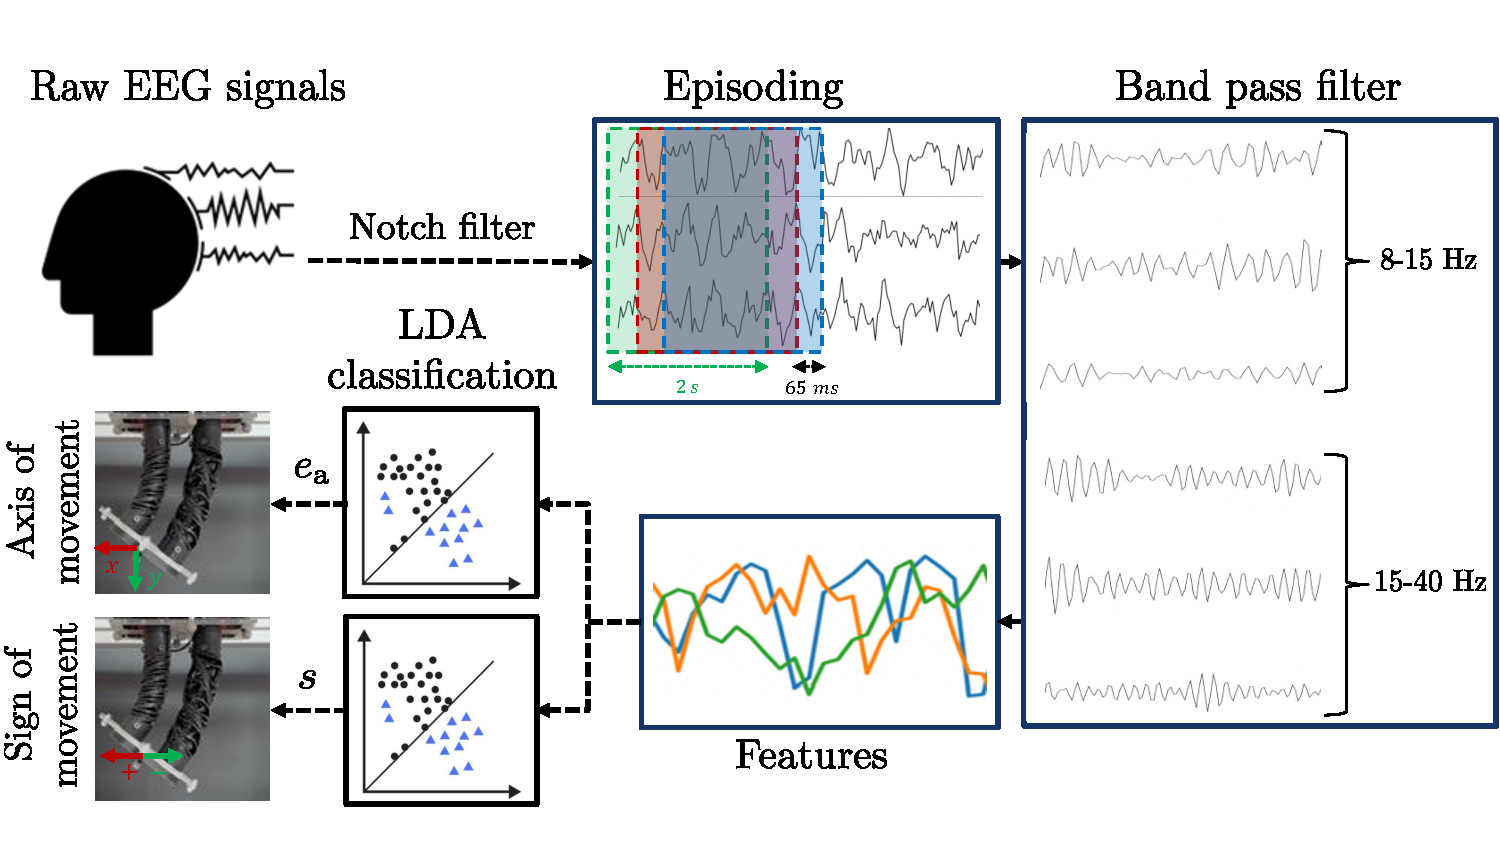
\includegraphics[width=\columnwidth]{braincontrol/figures/eeg_pipeline/eeg_pipeline_v3_compressed.pdf}
    \caption{EEG data processing pipeline: The EEG data is acquired in real-time, pre-processed, and divided into episodes and subbands. Next, we extract power features and pass them to two LDA classifiers: the first outputs the axis of movement (for example, moving along the x- or y-axis), and the second provides the sign of movement (for example, positive or negative movement along the active axis). These commands are then used to move the attractor in Cartesian space.}
    \label{fig:braincontrol:eeg_pipeline}
\end{center}
\end{figure}

\subsection{Computational Controller}\label{sub:braincontrol:computational_controller}
We adopt the Cartesian impedance controller from Sec.~\ref{sub:hsacontrol:task_space_impedance_control:control_strategy} to shape the potential field with a computational controller such that the attractor $x^\mathrm{at}$ becomes a globally asymptotically stable equilibrium
\begin{equation}\label{eq:braincontrol:cartesian_impedance_controller}
\begin{split}
    \tau =& \: J^\top(q) \, \left (K_x \, (x^\mathrm{at} - x) - D_x \, \dot{x} \right ) + G(q) + K \, (q-q^0)\\
    & \: + J^\top(q) \, J_\mathrm{M}^{+\top}(q) \, D \, \dot{q} + J^\top(q) \, \mu(q,\dot{q}) \left ( I_3 - J_\mathrm{M}^+(q) J(q) \right )\dot{q}.
\end{split}
\end{equation}

% \begin{figure}
%     \centering
%     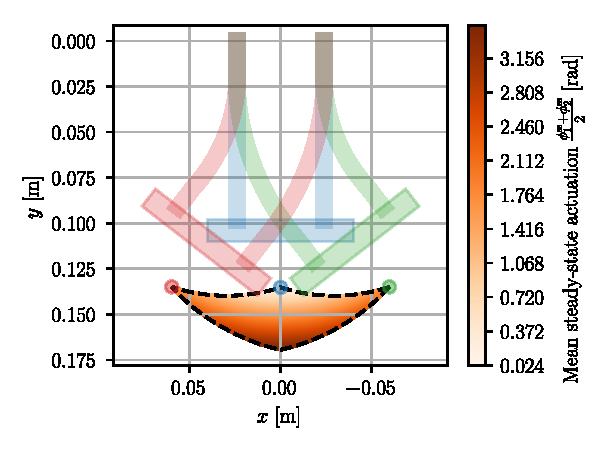
\includegraphics[width=0.85\columnwidth, trim={10 10 10 10}]{braincontrol/figures/workspace/operational_workspace_fpu_with_ee.pdf}
%     \caption{Operational workspace of a HSA robot with attached end-effector: the color displays the mean steady-state actuation $\frac{\phi_1^\mathrm{ss} + \phi_2^\mathrm{ss}}{2}$ necessary for the end-effector to remain at the position. Additionally, we visualize three example shapes: the straight configuration with $\phi^\mathrm{ss} = (0, 0)$ (blue), maximum clockwise bending with $\phi^\mathrm{ss} = (3.49, 0) \, \si{rad}$ (red), and maximum counter-clockwise bending with $\phi^\mathrm{ss} = (0, 3.49) \, \si{rad}$ (green).}
%     \label{fig:braincontrol:hsa_workspace}
% \end{figure}

\begin{figure*}
\begin{center}
    \subfigure[Operational workspace]{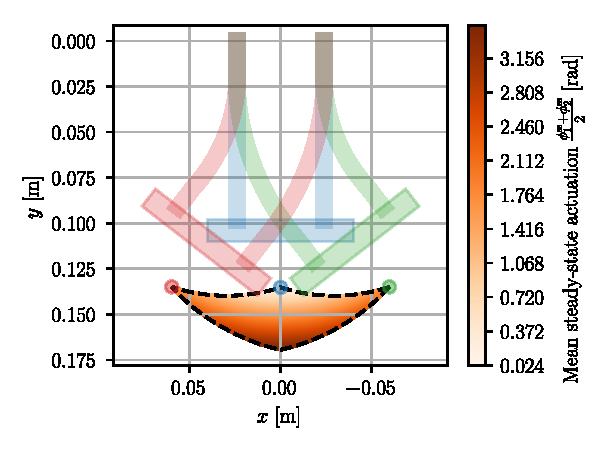
\includegraphics[width=0.36\linewidth]{braincontrol/figures/workspace/operational_workspace_fpu_with_ee.pdf}\label{fig:braincontrol:hsa_workspace}}
    \subfigure[Experimental setup]{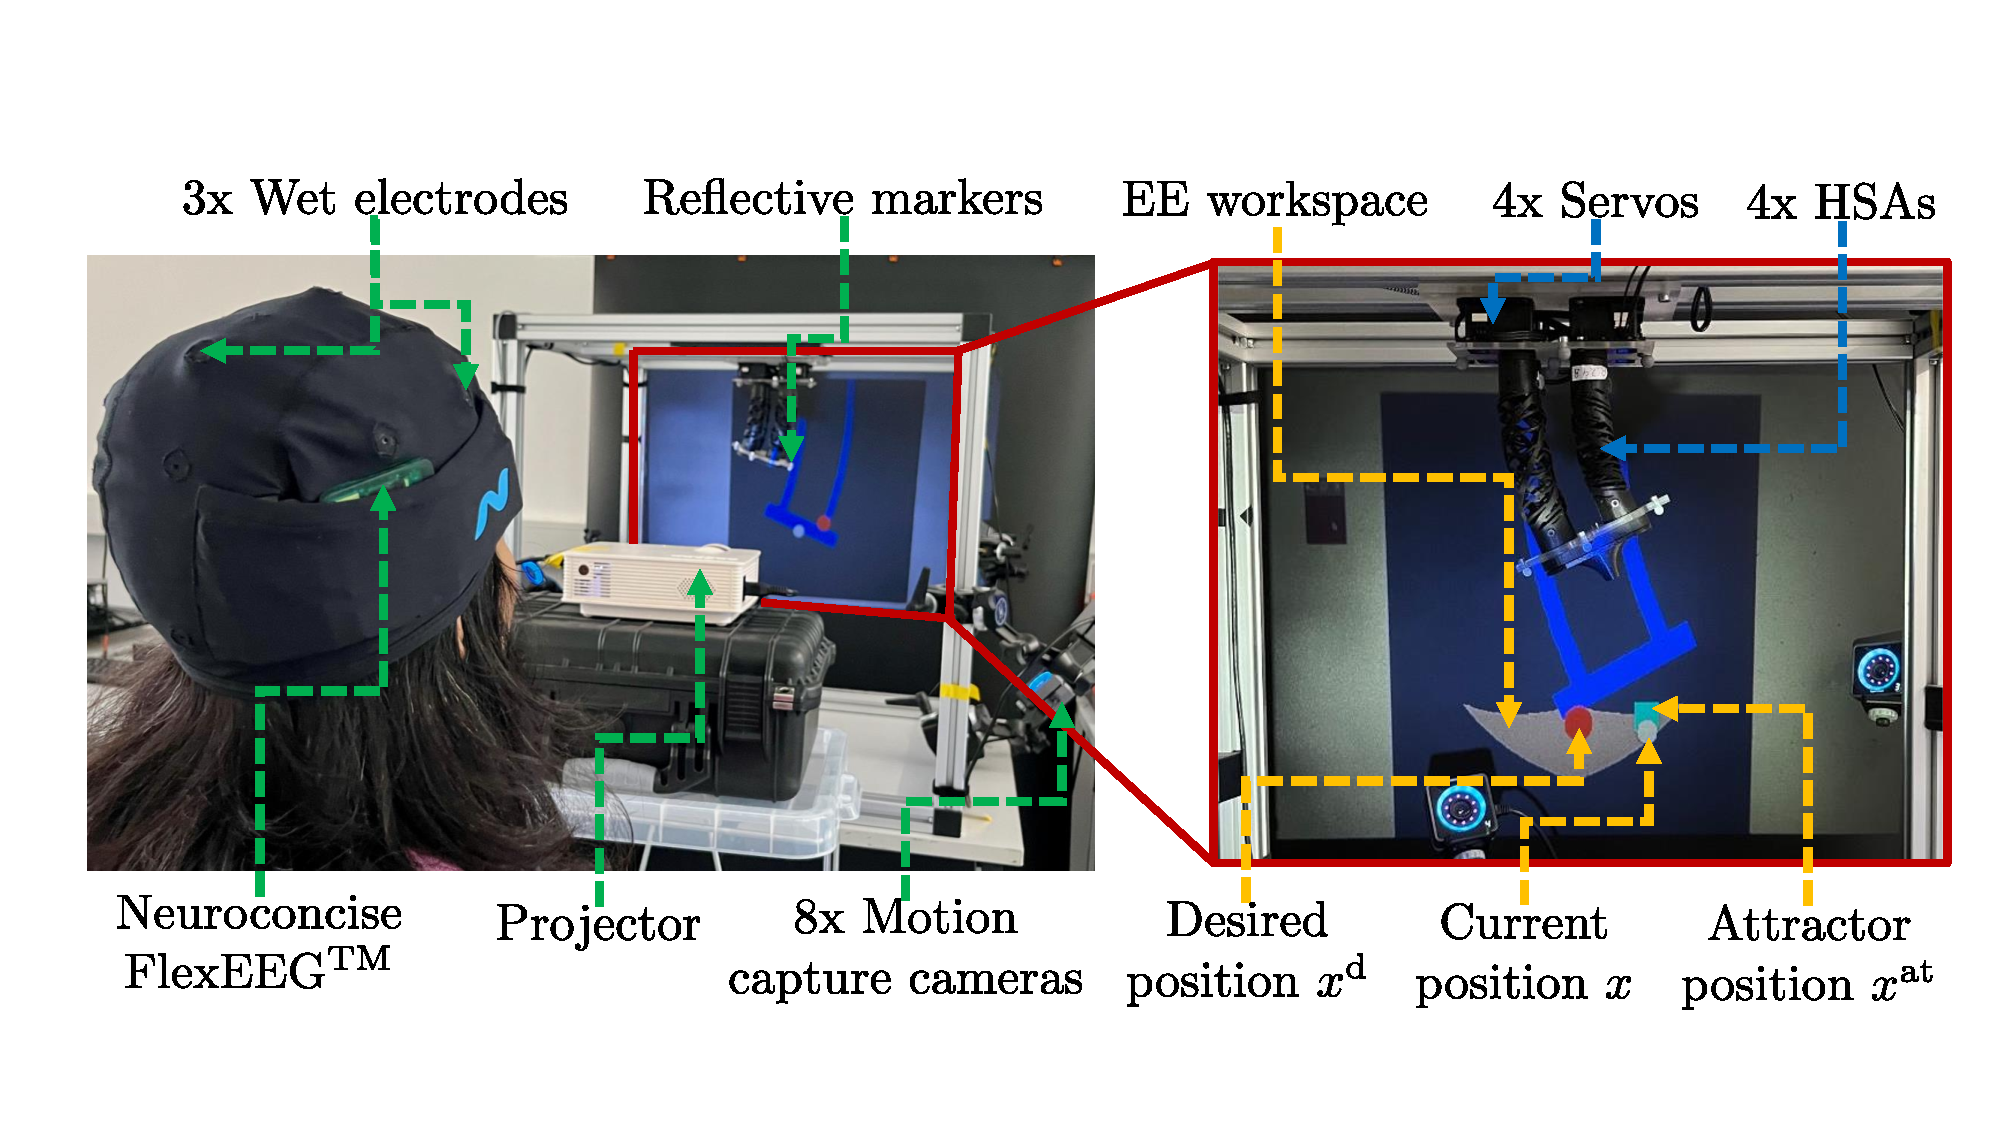
\includegraphics[width=0.63\linewidth]{braincontrol/figures/experimental_setup/experimental_setup_v3_cropped.pdf}\label{fig:braincontrol:experimental_setup}}
    \caption{\textbf{Panel (a:} Operational workspace of a HSA robot with attached end-effector: the color displays the mean steady-state actuation $\frac{\phi_1^\mathrm{ss} + \phi_2^\mathrm{ss}}{2}$ necessary for the end-effector to remain at the position. Additionally, we visualize three example shapes: the straight configuration with $\phi^\mathrm{ss} = (0, 0)$ (blue), maximum clockwise bending with $\phi^\mathrm{ss} = (3.49, 0) \, \si{rad}$ (red), and maximum counter-clockwise bending with $\phi^\mathrm{ss} = (0, 3.49) \, \si{rad}$ (green).
    \textbf{Panel (b):} The HSA robot is mounted platform-down to a motion capture cage with 8x Optitrack PrimeX 13 cameras, which track the 3D pose of the platform (i.e., the end-effector). A Dynamixel MX-28 servo actuates each of the four HSAs. We project a rendering of the current (white dot) and desired (red dot) end-effector position, the attractor (green square), and the operational workspace (grey area) onto the black screen in the background. The study subject wears a cap with the Neuroconcise FlexEEG sensor, and we acquire the data from three electrodes connected to the motor cortex.}
\end{center}
\end{figure*}

\begin{figure}
\begin{center}
    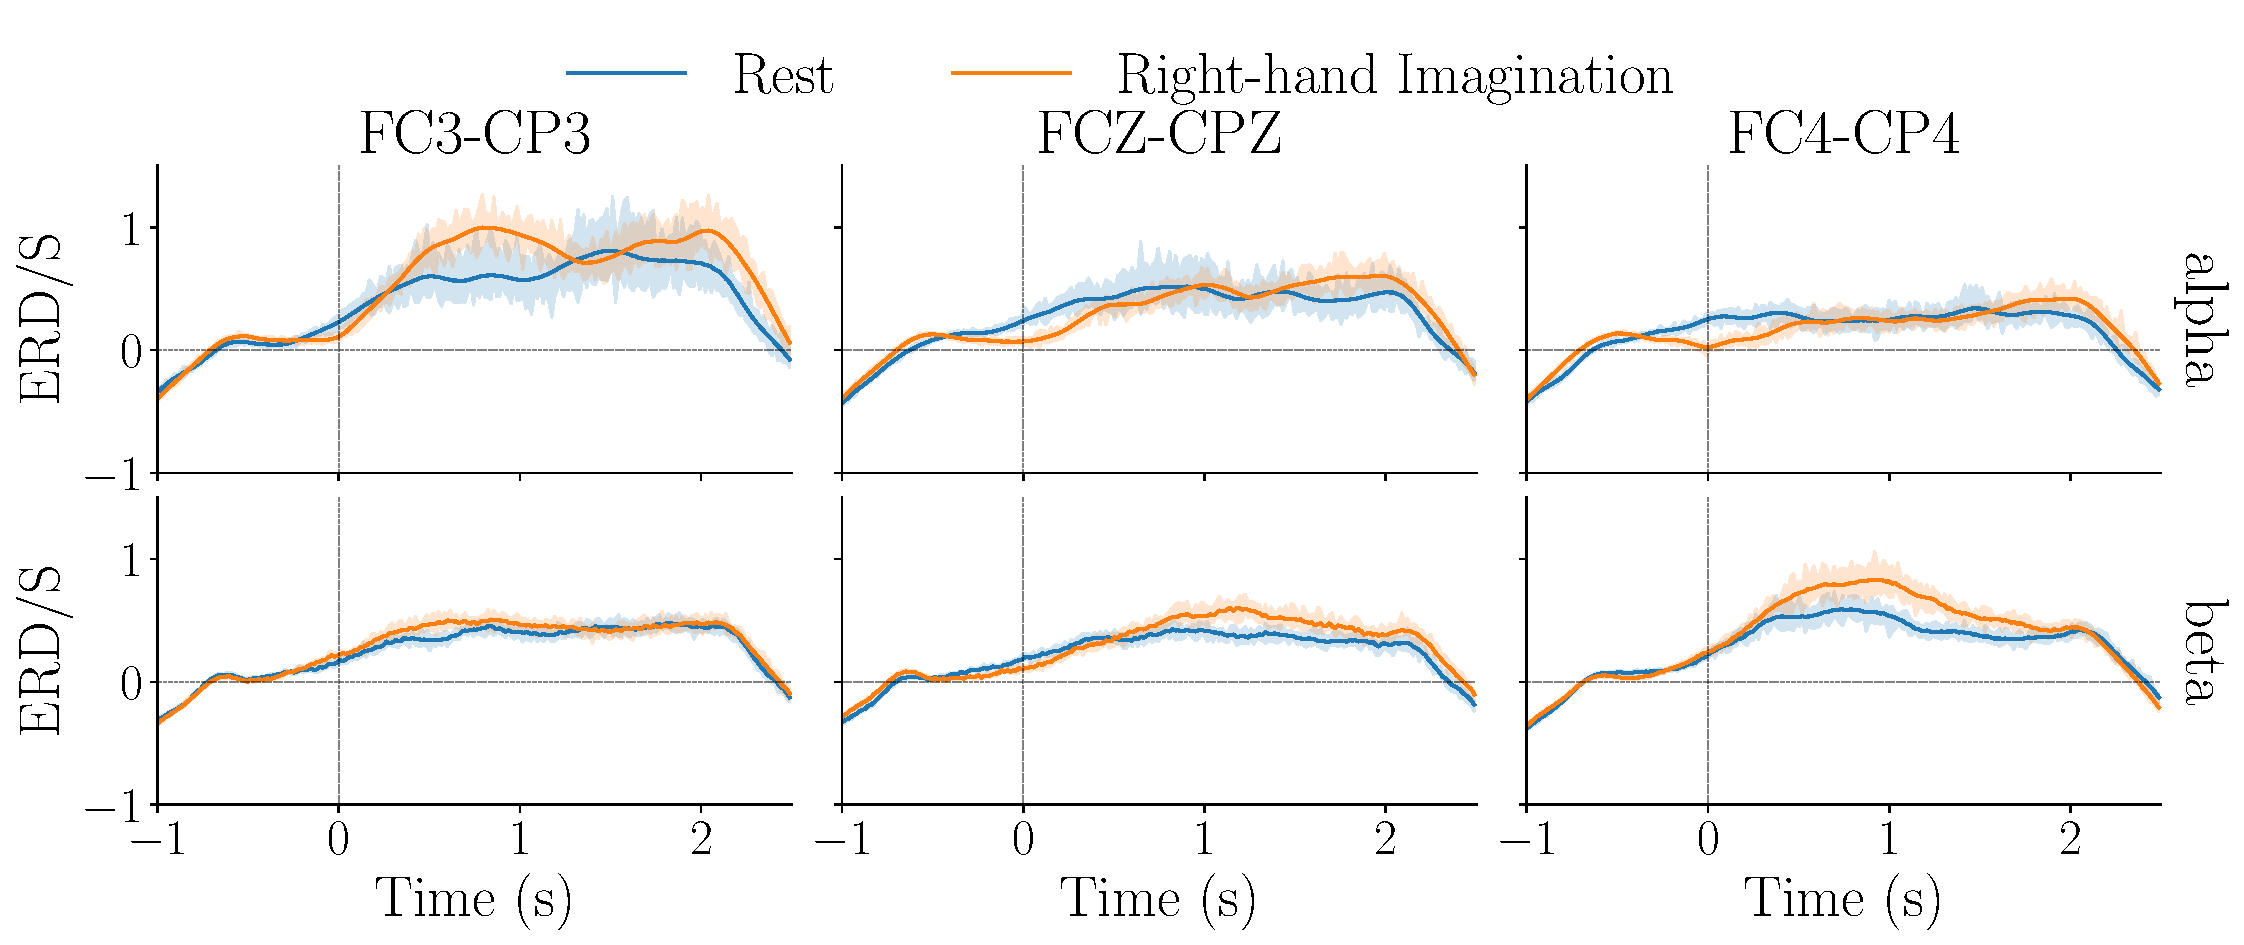
\includegraphics[width=0.85\columnwidth]{braincontrol/figures/eeg_pipeline/ERDS.pdf}
    \caption{ERD/S (overall average) over a time period of \SI{2.5}{s} of training data for right-hand Imagination v/s rest state including the Alpha and Beta bands of the EEG signals where the cue is presented at \SI{0}{s}. We plot the data of three sensors (i.e., channels): FC3-CP3 (left), FCZ-CPZ (middle), and FC4-CP4 (right).}
    \label{fig:braincontrol:ERDS}
\end{center}
\end{figure}

\begin{figure*}[t]
    \centering
    \subfigure[End-effector x-coordinate]{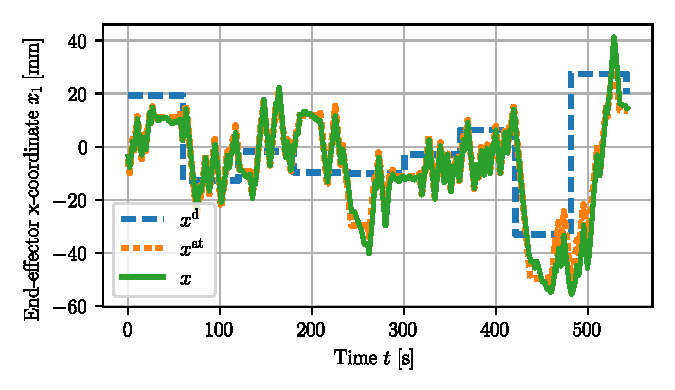
\includegraphics[width=0.47\textwidth, trim={5, 5, 5, 5}]{braincontrol/figures/setpoint_regulation/20231031_185546_pee_x.pdf}\label{fig:braincontrol:experimental_results:setpoint_regulation:brain:pee_x}}
    \subfigure[End-effector y-coordinate]{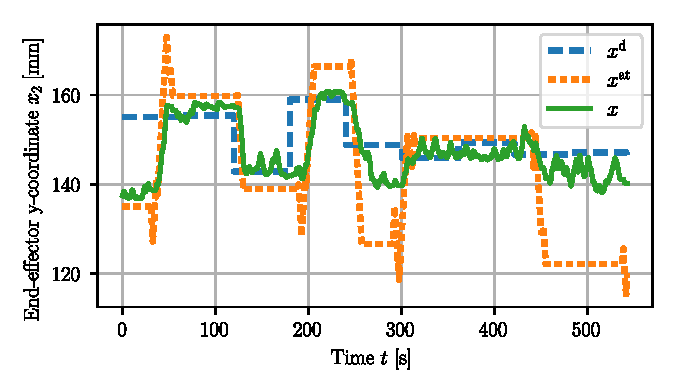
\includegraphics[width=0.47\textwidth, trim={5, 5, 5, 5}]{braincontrol/figures/setpoint_regulation/20231031_185546_pee_y.pdf}\label{fig:braincontrol:experimental_results:setpoint_regulation:brain:pee_y}}\\
    \subfigure[Configuration $q$]{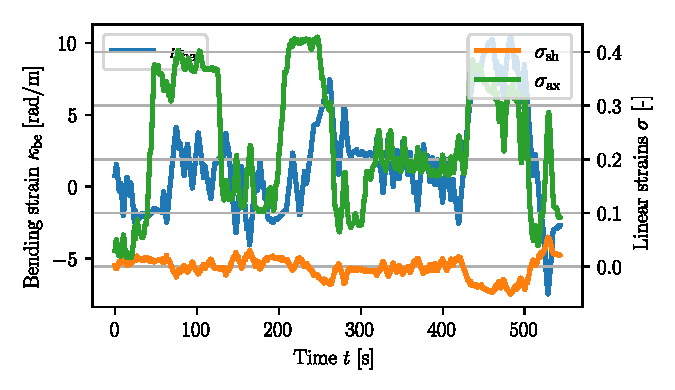
\includegraphics[width=0.47\textwidth, trim={5, 5, 5, 5}]{braincontrol/figures/setpoint_regulation/20231031_185546_q.pdf}\label{fig:braincontrol:experimental_results:setpoint_regulation:brain:q}}
    \subfigure[Control input $\phi$]{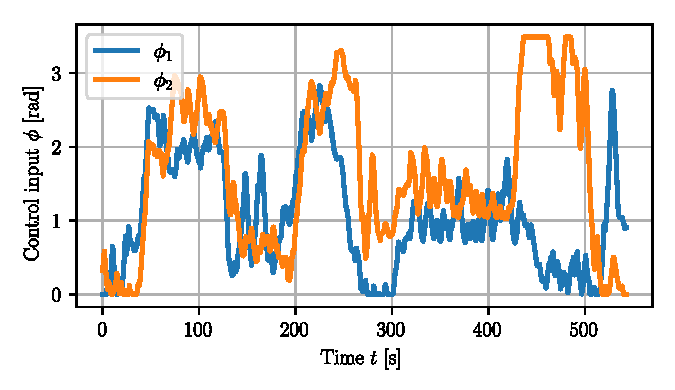
\includegraphics[width=0.47\textwidth, trim={5, 5, 5, 5}]{braincontrol/figures/setpoint_regulation/20231031_185546_phi.pdf}\label{fig:braincontrol:experimental_results:setpoint_regulation:brain:phi}}
    \caption{Experimental results for tracking a reference trajectory of nine-step functions with motor imagery. \textbf{Panel (a) \& (b):} The x/y-coordinate of the end-effector position with the solid line denoting the actual position, the dotted line the attractor position, and the dashed line the reference (i.e., the setpoint).
    \textbf{Panel (c):} The evolution of the configuration.
    \textbf{Panel(d):} The saturated planar control inputs. }\label{fig:braincontrol:experimental_results:setpoint_regulation:brain}
\end{figure*}